%%%%%%%%%%%%%%%%%%%%%%%%%%%%%%%%%%%%%%%%%%%%%%%%%%%%%%%%%%%%%%%%%%%%%%
%
% 都市システム工学科 特別研究概要テンプレート(H23 年度版)
%
%%%%%%%%%%%%%%%%%%%%%%%%%%%%%%%%%%%%%%%%%%%%%%%%%%%%%%%%%%%%%%%%%%%%%%

\documentclass[a4paper,10pt]{jarticle}
\usepackage[dvips]{graphicx}
\usepackage{amsmath}
\usepackage{setspace}

\textwidth      18.0cm
\textheight     27.0cm
\oddsidemargin  -1.0cm
\evensidemargin -1.0cm
\topmargin      -2.3cm
\footskip        0.5cm
\columnsep       2.5zw

\renewcommand{\baselinestretch}{0.95}
\pagestyle{empty}

\makeatletter
\def\section{\@startsection {section}{1}{\z@}{-3.5ex plus -1ex minus 
 -.2ex}{2.3ex plus .2ex}{\normalsize \bf}}
\def\subsection{\@startsection {subsection}{1}{\z@}{-3.5ex plus -1ex minus 
 -.2ex}{2.3ex plus .2ex}{\normalsize \bf}}
\makeatother

\begin{document}
\twocolumn[
\begin{center}
 \vspace{-2mm}
 \begin{large}
  {\bf システムツリー型モデルを利用した風力発電設備の安定運用計画の立案}
 \end{large}
 \vspace{-2mm}
\end{center}
 {\bf システム最適化研究室}
 \hfill {\bf シス05-19 臼木 誠}
 \vspace{5mm}
] % End of twocolumn

%% vspace のあとの寸法は,出来上がりイメージを見て適宜修正すること

%%%%%%%%%%%%%%%%%%%%%%%%%%%%%%%%%%%%%%%%%%%%%%%%%%%%%%%%%%%%%%%%%%%%%%
\vspace{-8mm}
\section{はじめに}
\vspace{-4mm}
%%%%%%%%%%%%%%%%%%%%%%%%%%%%%%%%%%%%%%%%%%%%%%%%%%%%%%%%%%%%%%%%%%%%%%

 日本では,東北地方太平洋沖地震での福島第一原子力発電所の事故によって原子力発電の危険性が再認識され,
原子力に変わる安全性のある新たなエネルギーとして,再生可能エネルギーが今まで以上に目が向けられている.

そこで本研究では,風力発電の出力変動を抑え,安定した電力の供給を行い,事業の利益も追求することを目的とした研究を行う.
前年度の卒業研究\cite{徳谷}では風を不完全情報として扱い,オンラインアルゴリズム的思考に基づいた運用計画の立案を行った.
本研究では,気象庁の過去の風況データを用いて,風速がどのようなパターンで変化するかの確率評価を行い,シナリオ・ツリー型モデルを
用いた運用計画を立案する.

%%%%%%%%%%%%%%%%%%%%%%%%%%%%%%%%%%%%%%%%%%%%%%%%%%%%%%%%%%%%%%%%%%%%%%
\vspace{-5mm}
\section{本研究の目的}
\vspace{-3mm}
%%%%%%%%%%%%%%%%%%%%%%%%%%%%%%%%%%%%%%%%%%%%%%%%%%%%%%%%%%%%%%%%%%%%%%

 本研究では,前年度の計画破綻の原因を考慮して,蓄電池の容量管理を主眼に置いた風力発電設備の運用計画を
数理計画法を用いて立案する.
風力発電の不安定な発電出力はシナリオ・ツリーを導入することによって,風速の確率評価を行い,発電出力の期待値を予想する.
今回も\cite{徳谷}と同様に出力一定制御型に対する運用計画の立案を行う.

本研究で提案する数理計画問題の目的関数は電力の売上高を最大化することであり,風力発電が事業として利益が出ているかも調べる.
このことから技術要件に沿った送電を行い,蓄電池の容量にも余裕を持たせつつ,極力電力を売るという戦略を取らなければならない.

%%%%%%%%%%%%%%%%%%%%%%%%%%%%%%%%%%%%%%%%%%%%%%%%%%%%%%%%%%%%%%%%%%%%%%
\vspace{-4mm}
\section{提案する数理計画モデル}
\vspace{-3.5mm}
%%%%%%%%%%%%%%%%%%%%%%%%%%%%%%%%%%%%%%%%%%%%%%%%%%%%%%%%%%%%%%%%%%%%%%

%%%%%%%%%%%%%%%%%%%%%%%%%%%%%%%%%%%%%%%%%%%%%%%%%%%%%%%%%%%%%%%%%%%%%%
\subsection{最適化モデルに必要な要素}
\vspace{-3.5mm}
%%%%%%%%%%%%%%%%%%%%%%%%%%%%%%%%%%%%%%%%%%%%%%%%%%%%%%%%%%%%%%%%%%%%%%
ここでは運用計画の最適化モデルに必要な記号について説明する.
\begin{spacing}{0.9}
\begin{itemize}
\item 集合・添字

\begin{itemize}
\item $t \in T$: 時刻を表す添字 $t$ とその集合 $T$
\item $s \in S$: シナリオを表す添字 $s$ とその集合 $S$
\end{itemize}

\item パラメータ
\begin{itemize}
\item $\tilde{s}_{ts}$: 時刻$t$におけるシナリオ$s$に対応する,時刻$t-1$におけるシナリオ番号
\item $r_t$: 時刻$t$における売電価格
\item $P_{ts}$: 時刻$t$におけるシナリオ$s$の発生確率
\item $w_{ts}$: 時刻$t$におけるシナリオ$s$での発電量
\item $CA$: 蓄電池容量
\item $\tilde{P}_U, \tilde{P}_L$: 風力発電設備の運用が破綻する確率の許容値.
\item $\tilde{C}_U, \tilde{C}_L$: 最終時刻における蓄電量の期待値の上下限
\item $H$: 蓄電池を作動温域になるためのヒータ損失
\item $m$: マージン係数
\item $M$: 非常に大きな正の定数
\end{itemize}
\item 変数
\begin{itemize}
\item $WB_t$: 時刻 $t$ において,WF(ウィンドファーム)で発電した電気のうち,蓄電池に蓄電される電気量の期待値
\item $WG_t$: 時刻 $t$ において,WFで発電した電気のうち,電力購入会社へ売電される電気量の期待値
\item $BG_t$: 時刻 $t$ において,蓄電池にある電気のうち,電力購入会社へ売電される電気量の期待値
\item $C_{ts}$: 時刻 $t$ におけるシナリオ $s$ においての蓄電量
\item $\delta^{1U}_{ts}, \delta^{1L}_{ts}, \delta^{2U}_{ts}, \delta^{2L}_{ts}$: 中間変数($0\mathchar`-1$ 変数)
\item $v^U_{ts}, v^L_{ts}$: 中間変数
\end{itemize}
\end{itemize}
\end{spacing}
%%%%%%%%%%%%%%%%%%%%%%%%%%%%%%%%%%%%%%%%%%%%%%%%%%%%%%%%%%%%%%%%%%%%%%
\vspace{-6mm}
\subsection{モデルの目的関数・制約条件}
\vspace{-3.5mm}
%%%%%%%%%%%%%%%%%%%%%%%%%%%%%%%%%%%%%%%%%%%%%%%%%%%%%%%%%%%%%%%%%%%%%%

ここでは,提案する数理計画モデルの目的関数と制約条件について説明する.

【目的関数】

本モデルの目的は,(本節で示す制約条件の下で)電力の売上高を最大化することである.
電力売上高は,次式のように書くことができる.
\vspace{-1mm}
\begin{spacing}{0.5}
\begin{align*}
\sum_{t = 1}^n r_t \cdot (WG_t + BG_t)
\end{align*}
\end{spacing}

【制約条件】
\vspace{-2mm}
\begin{spacing}{0.6}
\begin{align}
WB_t + WG_t &= \sum_{s \in S} P_{ts} w_{ts}
\label{al:1}
\end{align}
\end{spacing}

(\ref{al:1})は,時刻 $t$ におけるWFの発電量の期待値を示している.
WFで発電された電力は,電力購入会社へ送電され,発電量が計画値より過剰だった場合,その分蓄電池に送電するようになっている.

\begin{spacing}{0.6}
\begin{align*}
- M (1 - \delta^{1L}_{ts})  \le 0.98 (WG_t + BG_t) - w_{ts}  \le M \delta^{1L}_{ts}
\end{align*}
\footnotesize{
\begin{align*}
v^L_{ts} - M (1 - \delta^{1L}_{ts}) \le 0.98 (WG_t + BG_t) - w_{ts} \le v^L_{ts} + M (1 - \delta^{1L}_{ts})
\end{align*}
}
\normalsize
\begin{align*}
- M \delta^{1L}_{ts} \le v^L_{ts} \le M \delta^{1L}_{ts}
\end{align*}
\begin{align*}
- M (1 - \delta^{1U}_{ts}) \le w_{ts} - 1.02 (WG_t + BG_t) \le M \delta^{1U}_{ts}
\end{align*}
\footnotesize{
\begin{align*}
v^U_{ts} - M (1 - \delta^{1U}_{ts}) \le w_{ts} - 1.02 (WG_t + BG_t) \le v^U_{ts} + M (1 - \delta^{1U}_{ts})
\end{align*}
}
\normalsize
\begin{align*}
- M \delta^{1U}_{ts} \le v^U_{ts} \le M \delta^{1U}_{ts}
\end{align*}
\end{spacing}

これらの制約条件は,出力一定制御型の技術要件を表しており,合成出力が通告した計画値の$\pm2\%$を超えないようにしている.

\vspace{-2mm}
\begin{spacing}{0.6}
\begin{align}
C_{ts} = C_{t-1,\tilde{s}_{ts}} - \frac{1}{0.9} v^L_{ts} + 0.95 v^U_{ts} - H
\label{al:2}
\end{align}
\end{spacing}

(\ref{al:2})は,シナリオ$\tilde{s}_{ts}$から,時刻 $t$におけるシナリオ$s$への蓄電池の変化量を表している.

\begin{spacing}{0.6}
\begin{align}
- M (1 - \delta^{2L}_{ts}) \le m * CA - C_{ts} \le M \delta^{2L}_{ts}
\label{al:3}
\end{align}
\begin{align}
- M (1 - \delta^{2U}_{ts}) \le C_{ts} - m * CA \le M \delta^{2U}_{ts}
\label{al:4}
\end{align}
\end{spacing}

(\ref{al:3}),(\ref{al:4})は,蓄電池容量の上下限マージンを表す.

\begin{spacing}{0.6}
\begin{align}
\sum_{s \in S} \delta^{2L}_{ts} P_{ts} \le \tilde{P}_L
\label{al:5}
\end{align}
\begin{align}
\sum_{s \in S} \delta^{2U}_{ts} P_{ts} \le \tilde{P}_U
\label{al:6}
\end{align}
\end{spacing}

(\ref{al:5}),(\ref{al:6})は,時刻$t$における容量管理が出来ていないシナリオ$s$の発生確率の総和が,
蓄電池のマージンにおける上下限の発生確率の許容値を,超えないようにしている.

\begin{spacing}{0.6}
\begin{align}
\tilde{C}_L \le \sum_{s \in S} C_{ns} \le \tilde{C}_U
\label{al:7}
\end{align}
\end{spacing}

(\ref{al:7})は,最終時刻における蓄電量の期待値の上下限以内に,最終時刻の蓄電量が収まるようにするための制約条件である.

%%%%%%%%%%%%%%%%%%%%%%%%%%%%%%
\vspace{-4mm}
\section{数値実験}
\vspace{-14mm} 
%%%%%%%%%%%%%%%%%%%%%%%%%%%%%%
			
%%%%%%%%%%%%%%%%%%%%%%%%%%%%%%%%%%%%%%%%%%%%%%%%%%%%%%%%%%%%%%%%%%%%%%
\subsection{実験内容}
\vspace{-4mm}
%%%%%%%%%%%%%%%%%%%%%%%%%%%%%%%%%%%%%%%%%%%%%%%%%%%%%%%%%%%%%%%%%%%%%%
																			
 ここでは,本研究で行った数値実験の内容について説明する.

まず,本実験では,発電計画の通告時間,ならびに通告更新周期を $2$ 時間と設定した.
これは,風力発電設備が売電するときの標準的な設定である\cite{電力}.

また,本実験では,シナリオ・ツリーの分岐数と期間数を変え,実験を行う.
分岐数と期間数の設定は,本実験において重要な意味を持つ.
なぜなら,シナリオ・ツリーの葉の数,すなわち最終期におけるシナリオの数は,「(分岐数)の(期間数)乗」となる.
この量に支配される変数や制約の数が存在するため,分岐数や期間数を大きく設定しすぎると,
実用上意味のある時間では最適解を求めることが出来なくなる可能性がある.

%%%%%%%%%%%%%%%%%%%%%%%%%%%%%%%%%%%%%%%%%%%%%%%%%%%%%%%%%%%%%%%%%%%%%%
\vspace{-6mm}
\subsection{実験結果}
\vspace{-4mm}
%%%%%%%%%%%%%%%%%%%%%%%%%%%%%%%%%%%%%%%%%%%%%%%%%%%%%%%%%%%%%%%%%%%%%%

 ここでは,前節で説明した設定の下で行った数値実験の結果を示す.
図\ref{fig:C2_T3},図\ref{fig:C3_T4}は,各分岐数と期間数毎による蓄電池容量とマージン設定の違いによる売電収入の図とそれにかかった計算時間の平均と分散の表\ref{tb:2}である.


\begin{figure}[h]
\centering
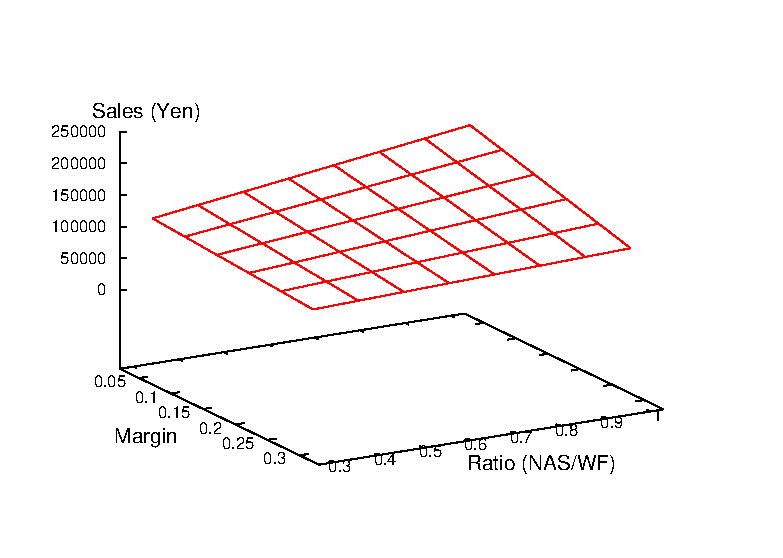
\includegraphics[width=7cm,height=4.5cm, clip]{stdout_C2_T3_data_m.eps}
\caption{2分岐,3期間の場合}
\label{fig:C2_T3}
\end{figure}

\begin{figure}[h]
\centering
\includegraphics[width=7cm,height=4.5cm, clip]{stdout_C3_T4_data_m.eps}
\caption{3分岐,4期間の場合}
\label{fig:C3_T4}
\end{figure}


\begin{table}[]
\begin{center}
  \caption{本実験における計算時間(s)の平均・分散}
  \label{tb:2}
  \scalebox{0.7}[0.9]{
  \begin{tabular}{|c|c|c|c|c|c|c|c|}
  \hline
  分岐数・期間数 & 2・3 & 2・4 & 2・5 & 2・6 & 3・3 & 3・4 & 4・3 \\
  \hline
  平均 & 0.34 & 8.45 & 192.94 & 1244.24 & 120.70 & 0.36 & 8.66 \\
  \hline
  分散 & 0.10 & 4.60 & 271.61 & 1211.01 & 96.50 & 0.16 & 4.73 \\
  \hline
  \end{tabular}
  }
\end{center}
\end{table}


図\ref{fig:C3_T4}で線が描かれていない場所は,最適解が得られなかったものである.
結果から見ると,分岐数や期間数が多くなっていくと最適解を得られないことが多くなった.
またマージン係数と蓄電池容量は,それぞれの最小値と最大値に近づくと最適解を得られにくい傾向にある.
表\ref{tb:2}における結果からは,分岐数と期間数における計算時間の増加の違いがみえる.
基本的には分岐数の増加による計算時間の平均・分散の増加は小さく,期間数の増加による計算時間の平均・分散の増加は大きい.

%%%%%%%%%%%%%%%%%%%%%%%%%%%%%%%%%%%%%%%%%%%%%%%%%%%%%%%%%%%%%%%%%%%%%%
\vspace{-6mm}
\subsection{考察}
\vspace{-2.5mm}
%%%%%%%%%%%%%%%%%%%%%%%%%%%%%%%%%%%%%%%%%%%%%%%%%%%%%%%%%%%%%%%%%%%%%%

 今回の実験結果から,WF の定格出力に対する蓄電池容量の比が同じであれば,マージン係数が小さい
(蓄電池容量に対して利用できる範囲が大きい)方が電力の売上高が大きくなるということがわかる.
一方,マージン係数が一定のとき,WF の定格出力に対する蓄電池容量の比を大きくしても,
必ずしも売上高は大きくならないという現象も確認することができる.
蓄電池の容量が大きい場合,蓄電できる容量は大きくなるわけだが,逆に蓄電池の温度維持に必要となる電力も大きいため,
必ずしも利益には結びつかないということだと考えられる.
今回の実験では予測値が $5.0$ (m/s) の場合を扱っているが,予測値(あるいは平均風速)がこれよりも大きい場合は,
また違った傾向が観察されるものと考えられる.

%%%%%%%%%%%%%%%%%%%%%%%%%%%%%%%%%%%%%%%%%%%%%%%%%%%%%%%%%%%%%%%%%%%%%%
\vspace{-6mm}
\section{おわりに}
\vspace{-3.5mm}
%%%%%%%%%%%%%%%%%%%%%%%%%%%%%%%%%%%%%%%%%%%%%%%%%%%%%%%%%%%%%%%%%%%%%%

 本研究では,風力発電の運用計画をシナリオ・ツリーを用いたモデル化を行い,数値実験で各種条件を変えても
安定した運用が継続できることを示した.

本研究では,出力一定制御型に対する運用計画の立案を行ったが,蓄電池併設風力発電には出力変動緩和型の制御型も提案されている.
今回は出力変動緩和型の運用計画の立案はできなかったが,こちらの安定運用の計画も立案し,出力一定制御型の運用計画との違いを
検証していくことが今後の課題と考える.

%文献や式・図表の引用は以下のように:
%\begin{itemize}
 %\item \cite{都市12}
 %\item 式 (\ref{eq:G})
 %\item 図 \ref{fig:1}
 %\item 表 \ref{tb:1}
%\end{itemize}

%%%%%%%%%%%%%%%%%%%%%%%%%%%%%%%%%%%%%%%%%%%%%%%%%%%%%%%%%%%%%%%%%%%%%%
\vspace{-4mm}
\begin{thebibliography}{9}
\vspace{-2.5mm}
%
\bibitem{電力}
谷川亮一,青木功,田邊隆之,電力ソリューション特集,2009\\
{\footnotesize (http://www.meidensha.co.jp/pages/tech/tech01/review-200903/article-200903-0051.pdf)}

\bibitem{徳谷}
徳谷祐貴,不完全情報化において風力発電を効率的に運用する計画の立案,2010

%	
\end{thebibliography}
%%%%%%%%%%%%%%%%%%%%%%%%%%%%%%%%%%%%%%%%%%%%%%%%%%%%%%%%%%%%%%%%%%%%%%

\end{document}
%\begin{table}
 %\begin{center}
  %\caption{表のタイトルは上に配置}
  %\begin{tabular}{|l|l|l|}
   %\hline
   %A \hspace{2cm} & B \hspace{2cm} & C \hspace{2cm} \\
   %\hline
   %あ & い & う \\
   %\hline
  %\end{tabular}
  %\label{tb:1}
 %\end{center}
%\end{table}
%%%%% End of file %%%%%